% This LaTeX document needs to be compiled with XeLaTeX.
\documentclass[
  10
]{article}
\usepackage[margin=2cm,includehead=true,includefoot=true,centering,]{geometry}
\usepackage{xcolor}
\usepackage{ucharclasses}
\usepackage{hyperref}
\usepackage{amsmath,amssymb}
\usepackage{amsfonts}
\usepackage[version=4]{mhchem}
\usepackage{stmaryrd}
\usepackage{bbold}
\usepackage{polyglossia}
\usepackage{fontspec}
\usepackage{ctex}
\usepackage[export]{adjustbox}
\usepackage{tabularx}
\usepackage{booktabs}

\usepackage{setspace}
\setstretch{1.2}

\makeatletter
\@ifundefined{KOMAClassName}{% if non-KOMA class
  \IfFileExists{parskip.sty}{%
    \usepackage{parskip}
  }{% else
    \setlength{\parindent}{0pt}
    \setlength{\parskip}{6pt plus 2pt minus 1pt}}
}{% if KOMA class
  \KOMAoptions{parskip=half}}
\makeatother
\usepackage{longtable,booktabs,array}
\newcounter{none} % for unnumbered tables
\usepackage{calc} % for calculating minipage widths
% Correct order of tables after \paragraph or \subparagraph
\usepackage{etoolbox}
\makeatletter
\patchcmd\longtable{\par}{\if@noskipsec\mbox{}\fi\par}{}{}
\makeatother
% Allow footnotes in longtable head/foot
\IfFileExists{footnotehyper.sty}{\usepackage{footnotehyper}}{\usepackage{footnote}}
\makesavenoteenv{longtable}
\usepackage{graphicx}
\makeatletter
\newsavebox\pandoc@box
\newcommand*\pandocbounded[1]{% scales image to fit in text height/width
  \sbox\pandoc@box{#1}%
  \Gscale@div\@tempa{\textheight}{\dimexpr\ht\pandoc@box+\dp\pandoc@box\relax}%
  \Gscale@div\@tempb{\linewidth}{\wd\pandoc@box}%
  \ifdim\@tempb\p@<\@tempa\p@\let\@tempa\@tempb\fi% select the smaller of both
  \ifdim\@tempa\p@<\p@\scalebox{\@tempa}{\usebox\pandoc@box}%
  \else\usebox{\pandoc@box}%
  \fi%
}
% Set default figure placement to htbp
\def\fps@figure{htbp}
\makeatother
\setlength{\emergencystretch}{3em} % prevent overfull lines
\providecommand{\tightlist}{%
  \setlength{\itemsep}{0pt}\setlength{\parskip}{0pt}}


\hypersetup{colorlinks=true, linkcolor=blue, filecolor=magenta, urlcolor=cyan,}
\urlstyle{same}

\usepackage{colortbl}
\definecolor{table-row-color}{HTML}{999999}
\definecolor{table-rule-color}{HTML}{999999}
%\arrayrulecolor{black!40}
\arrayrulecolor{table-rule-color}     % color of \toprule, \midrule, \bottomrule
\setlength{\aboverulesep}{0pt}
\setlength{\belowrulesep}{0pt}


\setotherlanguages{english}
\IfFontExistsTF{Source Han Serif CN}
{\newfontfamily\chinesefont{Source Han Serif CN}}
{\IfFontExistsTF{Noto Serif CJK SC}
  {\newfontfamily\chinesefont{Noto Serif CJK SC}}
  {\IfFontExistsTF{SimSun}
    {\newfontfamily\chinesefont{SimSun}}
    {\IfFontExistsTF{FangSong}
      {\newfontfamily\chinesefont{FangSong}}
      {\newfontfamily\chinesefont{Arial Unicode MS}}
}}}
\IfFontExistsTF{Times New Roman}
{\newfontfamily\englishfont{Times New Roman}}
{\IfFontExistsTF{Liberation Serif}
  {\newfontfamily\englishfont{Liberation Serif}}
  {\IfFontExistsTF{DejaVu Serif}
    {\newfontfamily\englishfont{DejaVu Serif}}
    {\newfontfamily\englishfont{Arial}}
}}


\author{}
\date{}

\begin{document}


\begin{enumerate}
\def\labelenumi{\arabic{enumi}.}
\setcounter{enumi}{4}
\tightlist
\item
  周庄共有 400 公顷耕地,
  秋季农作物的种植如图。结合两图可知周庄棉花的种植面积占总面积的( ),
  扇形统计图中 \(10 \%\) 所代表的农作物是( )。( )
\end{enumerate}

\pandocbounded{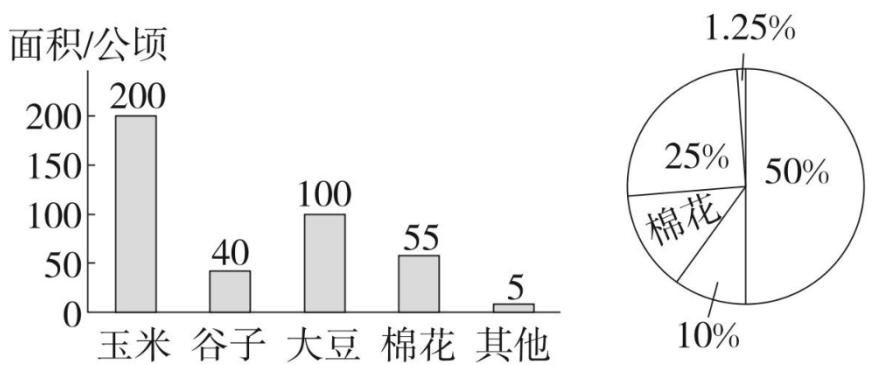
\includegraphics[keepaspectratio]{images/6cfdbb52e13a1c1d3639515a10221e3690a336175570c3ce7c17040703c37542.jpg}}

bar chart

\textbar{} 类别 \textbar{} 面积/公顷 \textbar{}
\textbar-\/-\/-\textbar-\/-\/-\textbar{} \textbar{} 玉米 \textbar{} 200
\textbar{} \textbar{} 谷子 \textbar{} 40 \textbar{} \textbar{} 大豆
\textbar{} 100 \textbar{} \textbar{} 棉花 \textbar{} 55 \textbar{}
\textbar{} 其他 \textbar{} 5 \textbar{} \textbar{} 类别 \textbar{} 数值
\textbar{} \textbar{} :-\/-\/- \textbar{} :-\/-\/- \textbar{} \textbar{}
玉米 \textbar{} 200 \textbar{} \textbar{} 谷子 \textbar{} 40 \textbar{}
\textbar{} 大豆 \textbar{} 100 \textbar{} \textbar{} 棉花 \textbar{} 55
\textbar{} \textbar{} 占比 (\%) \textbar{} 数值 \textbar{} \textbar{}
:-\/-\/- \textbar{} :-\/-\/- \textbar{} \textbar{} 玉米 \textbar{} 1.25
\textbar{} \textbar{} 谷子 \textbar{} 25 \textbar{} \textbar{} 大豆
\textbar{} 50 \textbar{} \textbar{} 棉花 \textbar{} 10 \textbar{}

A. 13.75\%,谷子

B. \(13\%\) ，谷子

C. 13.75\%, 棉花

D. 13.75\%, 大豆

\subsection{三、聪聪家 2018 年 5 月支出情况统计如下图,
其中该月的总支出是 3600 元。请你回答问题。(18
分)}\label{ux4e09ux806aux806aux5bb6-2018-ux5e74-5-ux6708ux652fux51faux60c5ux51b5ux7edfux8ba1ux5982ux4e0bux56fe-ux5176ux4e2dux8be5ux6708ux7684ux603bux652fux51faux662f-3600-ux5143ux8bf7ux4f60ux56deux7b54ux95eeux989818-ux5206}

\begin{enumerate}
\def\labelenumi{\arabic{enumi}.}
\item
  这个月哪项支出最多？支出了多少元？
\item
  文化教育支出了多少元？购买衣物支出了多少元？
\end{enumerate}

\pandocbounded{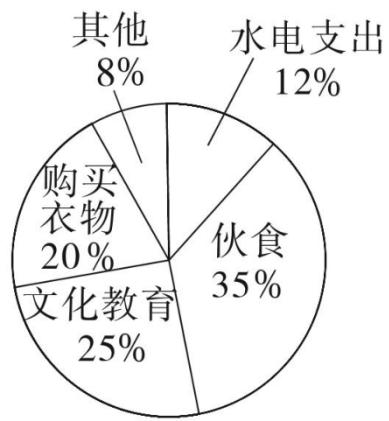
\includegraphics[keepaspectratio]{images/f3434658f67f323fc8ab3ddeba57c07124ed030ba139d29c057b2934c8466260.jpg}}

pie chart

\textbar{} 类别 \textbar{} 占比 (\%) \textbar{} \textbar{} :-\/-\/-
\textbar{} :-\/-\/- \textbar{} \textbar{} 水电支出 \textbar{} 12
\textbar{} \textbar{} 伙食 \textbar{} 35 \textbar{} \textbar{} 文化教育
\textbar{} 25 \textbar{} \textbar{} 购买衣物 \textbar{} 20 \textbar{}
\textbar{} 其他 \textbar{} 8 \textbar{}

\begin{enumerate}
\def\labelenumi{\arabic{enumi}.}
\setcounter{enumi}{2}
\tightlist
\item
  购买衣物的支出比文化教育支出少百分之几？少支出了多少元？
\end{enumerate}

\subsection{四、阳光食品公司 2018 年上半年生产情况统计图。(18
分)}\label{ux56dbux9633ux5149ux98dfux54c1ux516cux53f8-2018-ux5e74ux4e0aux534aux5e74ux751fux4ea7ux60c5ux51b5ux7edfux8ba1ux56fe18-ux5206}

\pandocbounded{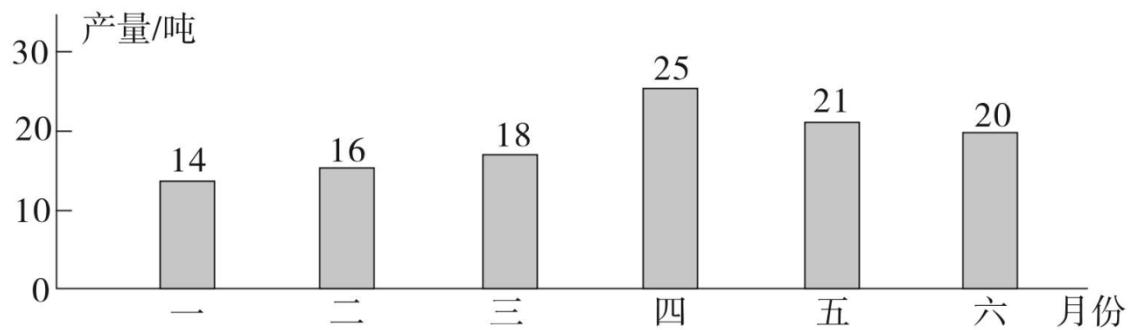
\includegraphics[keepaspectratio]{images/da68fcc32b230bb2d8478a2c936701d2c9521464888234035e1fe01c8ff5c2a7.jpg}}

bar chart

\textbar{} 月份 \textbar{} 产量/吨 \textbar{} \textbar{} :-\/-\/-
\textbar{} :-\/-\/- \textbar{} \textbar{} 一 \textbar{} 14 \textbar{}
\textbar{} 二 \textbar{} 16 \textbar{} \textbar{} 三 \textbar{} 18
\textbar{} \textbar{} 四 \textbar{} 25 \textbar{} \textbar{} 五
\textbar{} 21 \textbar{} \textbar{} 六 \textbar{} 20 \textbar{}

\begin{enumerate}
\def\labelenumi{\arabic{enumi}.}
\item
  ( )月份的产量最高，( )月份的产量最低。
\item
  上半年月平均产量是多少吨?
\item
  六月份产量比二月份增长百分之几?
\end{enumerate}

\subsection{五、琳琳将去年本地区上半年月平均气温做了如下统计:(10
分)}\label{ux4e94ux7433ux7433ux5c06ux53bbux5e74ux672cux5730ux533aux4e0aux534aux5e74ux6708ux5e73ux5747ux6c14ux6e29ux505aux4e86ux5982ux4e0bux7edfux8ba110-ux5206}

{\def\LTcaptype{none} % do not increment counter
\begin{longtable}[]{@{}|l|l|l|l|l|l|l|@{}}
\toprule\noalign{}
\endhead
\bottomrule\noalign{}
\endlastfoot
\hline
月份 & 1 & 2 & 3 & 4 & 5 & 6 \\
\hline
气温/°C & 0 & 1 & 2 & 7 & 12 & 18.5 \\
\hline
\end{longtable}
}

根据统计表完成下面统计图。

\pandocbounded{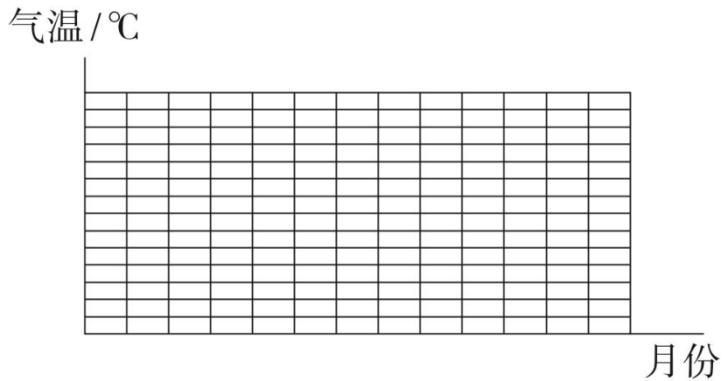
\includegraphics[keepaspectratio]{images/16b9558b3c5952c9ca2c32efd80f8a147c3fc863d2facc0cf13d5276d6ec254d.jpg}}

line chart

气温/℃ 月份 \textbar{} 月份 \textbar{} 气温 (℃) \textbar{}
\textbar-\/-\/-\textbar-\/-\/-\textbar{} \textbar{} 1月 \textbar{} 0
\textbar{} \textbar{} 2月 \textbar{} 0 \textbar{} \textbar{} 3月
\textbar{} 0 \textbar{} \textbar{} 4月 \textbar{} 0 \textbar{}
\textbar{} 5月 \textbar{} 0 \textbar{} \textbar{} 6月 \textbar{} 0
\textbar{} \textbar{} 7月 \textbar{} 0 \textbar{} \textbar{} 8月
\textbar{} 0 \textbar{} \textbar{} 9月 \textbar{} 0 \textbar{}
\textbar{} 10月 \textbar{} 0 \textbar{} \textbar{} 11月 \textbar{} 0
\textbar{} \textbar{} 12月 \textbar{} 0 \textbar{} \textbar{} 1月
\textbar{} 0 \textbar{} \textbar{} 2月 \textbar{} 0 \textbar{}
\textbar{} 3月 \textbar{} 0 \textbar{} \textbar{} 4月 \textbar{} 0
\textbar{} \textbar{} 5月 \textbar{} 0 \textbar{} \textbar{} 6月
\textbar{} 0 \textbar{} \textbar{} 7月 \textbar{} 0 \textbar{}
\textbar{} 8月 \textbar{} 0 \textbar{} \textbar{} 9月 \textbar{} 0
\textbar{} \textbar{} 10月 \textbar{} 0 \textbar{} \textbar{} 11月
\textbar{} 0 \textbar{} \textbar{} 12月 \textbar{} 0 \textbar{}

附加题。(10 分)

如图是小明家四月份支出及储蓄情况统计图。

\pandocbounded{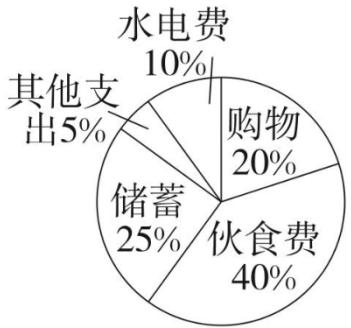
\includegraphics[keepaspectratio]{images/eb4004067f55bc9965b972fc2f9c12de687db1f86c40de1fba9de9a6e61264ea.jpg}}

pie chart

\textbar{} 类别 \textbar{} 占比 (\%) \textbar{}
\textbar-\/-\/-\textbar-\/-\/-\textbar{} \textbar{} 水电费 \textbar{} 10
\textbar{} \textbar{} 购物 \textbar{} 20 \textbar{} \textbar{} 伙食费
\textbar{} 40 \textbar{} \textbar{} 储蓄 \textbar{} 25 \textbar{}
\textbar{} 其他支出 \textbar{} 5 \textbar{}

\begin{enumerate}
\def\labelenumi{\arabic{enumi}.}
\item
  小明家四月份的伙食费共花了 800 元, 小明家的总支出及储蓄分别是多少元?
\item
  根据扇形统计图, 把下表填写完整。
\end{enumerate}

{\def\LTcaptype{none} % do not increment counter
\begin{longtable}[]{@{}|l|l|l|l|l|l|l|@{}}
\toprule\noalign{}
\endhead
\bottomrule\noalign{}
\endlastfoot
\hline
项目 & 伙食费 & 购物 & 水电费 & 储蓄 & 其他支出 & 总计 \\
\hline
费用/元 & 800 & & & & & \\
\hline
百分比 & 40\% & & & & & \\
\hline
\end{longtable}
}

\pandocbounded{
\includegraphics[keepaspectratio]{images/0178d070d62a17fb69e17e4642b89efdae64e5a979197bbccbde0442c75a4e09.jpg}}

\end{document}
